\documentclass{article}
\usepackage[utf8]{inputenc}
\usepackage[margin=1in]{geometry}
\usepackage{soul,color}
\usepackage{amsfonts, amsmath, amssymb}
\usepackage{bbm}
\usepackage{enumitem}
\usepackage[nobreak=true]{mdframed}
\usepackage{notes}
\usepackage{graphicx}
\usepackage{minted}

\newcommand{\solution}{\textbf{Solution: }}
\renewcommand{\N}{\mathcal{N}}
\newcommand{\Pbf}{\textbf{P}}
\renewcommand{\R}{\mathbb{R}}
\newcommand{\E}{\mathbb{E}}
\newcommand{\Var}{\text{Var}}
\newcommand{\Cov}{\text{Cov}}
\DeclareMathOperator{\p}{\text{P}}
\let\L\relax
\DeclareMathOperator{\L}{\mathcal{L}}
\let\l\relax
\DeclareMathOperator{\l}{\ell}
\renewcommand{\hat}{\widehat}

\title{CS189, HW3: Gaussians}
\author{ddavison@berkeley.edu}
% \date{January 2017}
\date{}

\begin{document}

\maketitle

\subsection*{1. Independence vs. Correlation}
\begin{enumerate}[label=(\alph*)]
    \item Consider the random variables $X, Y \in \R$ with the following conditions.
    \begin{enumerate}[label=(\roman*)]
        \item $X$ and $Y$ can take values $\{-1, 0, 1\}$.
        \item Either $X$ is 0 with probability $(\frac{1}{2})$, or $Y$ is 0 with probability $(\frac{1}{2})$.
        \item When $X$ is 0, $Y$ takes values 1 and -1 with equal probability $(\frac{1}{2})$. When $Y$ is 0, $X$ takes values 1 and -1 with equal probability $(\frac{1}{2})$.
    \end{enumerate}

    Are $X$ and $Y$ uncorrelated? Are $X$ and $Y$ independent? Prove your
    assertions. \emph{Hint:} Graph these points in the plane. What’s each
    point’s joint probability?

    \begin{mdframed}
      The information we are given corresponds to the following entries in a
      joint probability distribution table.

      \begin{tabular}{c | c | c | c | c | c}
        &    &     & Y   &     & \\
        &    &  -1 & 0   &   1 & \\
        \hline
        & -1 &     & 1/4 &     & \\
        X &  0 & 1/4 &     & 1/4 & 1/2 \\
        &  1 &     & 1/4 &     & \\
        \hline
        &    &     & 1/2 &     & \\
      \end{tabular}

      Using the fact that the rows and columns must sum to the marginal totals,
      and that each margin must sum to one, we can fill out the full joint
      distribution:

      \begin{tabular}{c | c | c | c | c | c}
        &    &     & Y   &     & \\
        &    &  -1 & 0   &   1 & \\
        \hline
        & -1 & 0   & 1/4 & 0   & 1/4\\
      X &  0 & 1/4 & 0   & 1/4 & 1/2 \\
        &  1 &  0  & 1/4 & 0   & 1/4 \\
        \hline
        &    & 1/4 & 1/2 & 1/4 & 1 \\
      \end{tabular}

% |   |    |     | Y   |     |     |
% |   |    |  -1 | 0   |   1 |     |
% |   | -1 |     | 1/4 |     |     |
% | X |  0 | 1/4 |     | 1/4 | 1/2 |
% |   |  1 |     | 1/4 |     |     |
% |   |    |     | 1/2 |     |     |

      We have
      \begin{align*}
        \E[X] = \mu_X =
        -1 \times \frac{1}{4} +
        0 \times \frac{1}{2} +
        1 \times \frac{1}{4}
        = 0,
      \end{align*}
      and $\E[Y] = \mu_Y = \mu_X$ because the marginal distributions of $X$ and $Y$ are identical.

    \end{mdframed}

    \begin{mdframed}
      \textbf{Are $X$ and $Y$ uncorrelated?} Yes. The definition of
      ``uncorrelated'' is that their covariance is zero. Their covariance is
      \begin{align*}
        \Cov(X, Y) = \E~ (X - \E[X])(Y - \E[Y]) = \E[XY] - \mu_X\mu_Y.
      \end{align*}
      But note that $\mu_X\mu_Y = 0 \cdot 0 = 0$, and for every sample point
      with non-zero probability, it is true that either $X = 0$ or $Y =
      0$. Therefore $\Cov(X, Y) = 0$; $X$ and $Y$ are uncorrelated.
    \end{mdframed}

    \begin{mdframed}
      \textbf{Are $X$ and $Y$ independent?} No. The definition of
      ``independent'' is that $Y$ contributes no information about $X$ (and
      equivalently, $X$ contributes no information about $Y$). More formally,
      $X$ and $Y$ are independent if and only if
      \begin{align*}
        \p(X=x|Y=y) &= \p(X=x)
      \end{align*}
      for every pair $(x, y)$.

      But this means that the columns of the joint probability distribution are
      identical (and hence the rows also). Since that is not the case, $X$ and
      $Y$ are not independent.


    \end{mdframed}


  \item Consider three Bernoulli random variables $B, C,$ and $D$ which take
    values $\{0, 1\}$ with equal probability. Construct three more random
    variables $X, Y, Z$ such that $X = B \oplus C, Y = C \oplus D$, and
    $Z = B \oplus D$, where $\oplus$ is the XOR (exclusive or) operator. Are
    $X, Y,$ and $Z$ pairwise independent? Mutually independent? Prove it.

    \begin{mdframed}
      % Intuitively, it seems that they are not pairwise independent for the
      % following reason: pairwise independence would require that
      % $\p(Z|X) = \p(Z)$.

      \begin{tabular}{c|c|c|c|c|c|c}
        B & C & D & X & Y & Z & Probability\\
        \hline
        0 & 0 & 0 & 0 & 0 & 0 & 1/8 \\
        0 & 0 & 1 & 0 & 1 & 1 & 1/8 \\
        0 & 1 & 0 & 1 & 1 & 0 & 1/8 \\
        0 & 1 & 1 & 1 & 0 & 1 & 1/8 \\
        1 & 0 & 0 & 1 & 0 & 1 & 1/8 \\
        1 & 0 & 1 & 1 & 1 & 0 & 1/8 \\
        1 & 1 & 0 & 0 & 1 & 1 & 1/8 \\
        1 & 1 & 1 & 0 & 0 & 0 & 1/8 \\
      \end{tabular}
      % | B | C | D | X | Y | Z |
      % | 0 | 0 | 0 | 0 | 0 | 0 |
      % | 0 | 0 | 1 | 0 | 1 | 1 |
      % | 0 | 1 | 0 | 1 | 1 | 0 |
      % | 0 | 1 | 1 | 1 | 0 | 1 |
      % | 1 | 0 | 0 | 1 | 0 | 1 |
      % | 1 | 0 | 1 | 1 | 1 | 0 |
      % | 1 | 1 | 0 | 0 | 1 | 1 |
      % | 1 | 1 | 1 | 0 | 0 | 0 |
    \end{mdframed}

    \begin{mdframed}
      \textbf{Are $X, Y,$ and $Z$ pairwise independent?} Yes.

      We have $\p(X=1) = \p(Y=1) = \p(Z=1) = 1/2$. Since all three have
      non-zero probability there's no risk on conditioning on an impossible
      event, and we can take the definition of pairwise independence to be:
      $X, Y,$ and $Z$ are pairwise independent if and only if
      \begin{align*}
        \p(X=1|Y) &= \p(X=1)\\
        \p(X=1|Z) &= \p(X=1)\\
        \p(Y=1|Z) &= \p(Y=1).
      \end{align*}
      Consider $X$ conditioned on $Y$. Of the events for which $Y=0$, half have
      $X=0$ and half have $X=1$. Similarly, of the events (rows) for which
      $Y=1$, half have $X=0$ and half have $X=1$. Therefore
      $\p(X=1|Y) = \p(X=1) = 1/2$. By the symmetry of the problem, the same is
      true for $\p(X=1|Z)$ and $\p(Y=1|Z)$. Therefore $X$, $Y$, and $Z$ are
      pairwise independent.
    \end{mdframed}

    \begin{mdframed}
      \textbf{Are $X, Y,$ and $Z$ mutually independent?} No.

      We can take the definition of mutual independence to be: $X, Y,$ and $Z$
      are mutually independent if and only if
      \begin{align*}
        \p(X=1|Y,Z) &= \p(X=1)\\
        \p(Y=1|X,Z) &= \p(Y=1)\\
        \p(Z=1|X,Y) &= \p(Z=1).
      \end{align*}

      It suffices to exhibit one counter-example. Consider conditioning on
      $Y=1,Z=1$. Of the events (rows) for which that is true, $X$ is always
      0. Therefore $\p(X=1|Y,Z) = 0 \neq \p(X=1)$.

    \end{mdframed}

\end{enumerate}

\newpage
\subsection*{2. Isocontours of Normal Distributions}
Let $f(\mu, \Sigma)$ be the density function of a normally distributed random variable in $\R^2$. Plot isocontours of the following functions.
\begin{enumerate}[label=(\alph*)]
    \item $f(\mu, \Sigma)$, where $\mu = \begin{bmatrix}1 \\ 1 \end{bmatrix}$ and $\Sigma = \begin{bmatrix} 1 & 0  \\ 0 & 2 \end{bmatrix}$.
    \begin{mdframed} \solution
    % SOLUTION HERE
    \end{mdframed}

    \item $f(\mu, \Sigma)$, where $\mu = \begin{bmatrix}-1 \\ 2 \end{bmatrix}$ and $\Sigma = \begin{bmatrix} 2 & 1  \\ 1 & 3 \end{bmatrix}$.
    \begin{mdframed} \solution
    % SOLUTION HERE
    \end{mdframed}

    \item $f(\mu_1, \Sigma_1) - f(\mu_2, \Sigma_2)$, where $\mu_1 = \begin{bmatrix} 0 \\ 2 \end{bmatrix}, \mu_2 = \begin{bmatrix} 2 \\ 0 \end{bmatrix}$ and $\Sigma_1 = \Sigma_2 = \begin{bmatrix} 2 & 1 \\ 1 & 1 \end{bmatrix}$.
    \begin{mdframed} \solution
    % SOLUTION HERE
    \end{mdframed}

    \item $f(\mu_1, \Sigma_1) - f(\mu_2, \Sigma_2)$, where $\mu_1 = \begin{bmatrix} 0 \\ 2 \end{bmatrix}, \mu_2 = \begin{bmatrix} 2 \\ 0 \end{bmatrix}, \Sigma_1 = \begin{bmatrix} 2 & 1 \\ 1 & 1 \end{bmatrix}$ and $\Sigma_2 = \begin{bmatrix} 2 & 1 \\ 1 & 3 \end{bmatrix}$.
    \begin{mdframed} \solution
    % SOLUTION HERE
    \end{mdframed}

    \item $f(\mu_1, \Sigma_1) - f(\mu_2, \Sigma_2)$, where $\mu_1 = \begin{bmatrix} 1 \\ 1 \end{bmatrix}, \mu_2 = \begin{bmatrix} -1 \\ -1 \end{bmatrix}, \Sigma_1 = \begin{bmatrix} 2 & 0 \\ 0 & 1 \end{bmatrix}$ and $\Sigma_2 = \begin{bmatrix} 2 & 1 \\ 1 & 2 \end{bmatrix}$.
    \begin{mdframed} \solution
    % SOLUTION HERE
    \end{mdframed}

\end{enumerate}

\newpage
\subsection*{3. Eigenvectors of the Gaussian Covariance Matrix}
Consider two one-dimensional random variables $X_1 \sim \N(3, 9)$ and $X_2 \sim \frac{1}{2}X_1 + \N(4, 4)$, where $\N(\mu, \sigma^2)$  is a Gaussian distribution with mean $\mu$ and variance $\sigma^2$. In software, draw $N = 100$ random two-dimensional sample points from $(X_1, X_2)$ such that the $i$th value sampled from $X_2$ is calculated based on the $i$th value sampled from $X_i$.
\begin{enumerate}[label=(\alph*)]
  \begin{mdframed}
    \begin{minted}{python}
      from numpy.random import normalxxx

      X1 = normal(3, 3, 100)
      X2 = X1/2 + normal(4, 2, 100)
      X = np.stack([X1, X2], axis=1)
      n, d = X.shape
    \end{minted}
  \end{mdframed}
\item Compute the mean (in $\R^2$) of the sample.
  \begin{mdframed}
    \begin{minted}{python}
      mu = X.mean(axis=0)
    \end{minted}
  \end{mdframed}

\item Compute the $2 \times 2$ covariance matrix of the sample.
  \begin{mdframed}
    \begin{minted}{python}
    Sigma = (X - mu).T @ (X - mu) / (n * d)
  \end{minted}
  \end{mdframed}

\item Compute the eigenvectors and eigenvalues of this covariance matrix.
  \begin{mdframed}
    \begin{minted}{python}
    from numpy.linalg import eigh
    evals, evecs = eigh(Sigma)
  \end{minted}
  \end{mdframed}

\item On a two-dimensional grid with a horizontal axis for $X_1$ with range $[-15, 15]$ and a vertical axis for $X_2$ with range $[-15, 15]$, plot
  \begin{enumerate}[label=(\roman*)]
  \item all $N=100$ data points, and
  \item arrows representing both covariance eigenvectors. The eigenvector arrows should originate at the mean and have magnitudes equal to their corresponding eigenvalues.
  \end{enumerate}
  \begin{mdframed}
    \begin{minted}{python}
      fig = plt.figure(figsize=(10,10))
      plt.xlim(-15,15)
      plt.ylim(-15,15)
      plt.scatter(X[:,0], X[:,1])
      arrow_kwargs = dict(fc="k", ec="k", head_width=0.3, head_length=0.5)
      plt.arrow(mu[0], mu[1],
                evecs[:,0][0] * evals[0],
                evecs[:,0][1] * evals[0],
                **arrow_kwargs)
      plt.arrow(mu[0], mu[1],
                evecs[:,1][0] * evals[1],
                evecs[:,1][1] * evals[1],
                **arrow_kwargs)
    \end{minted}
    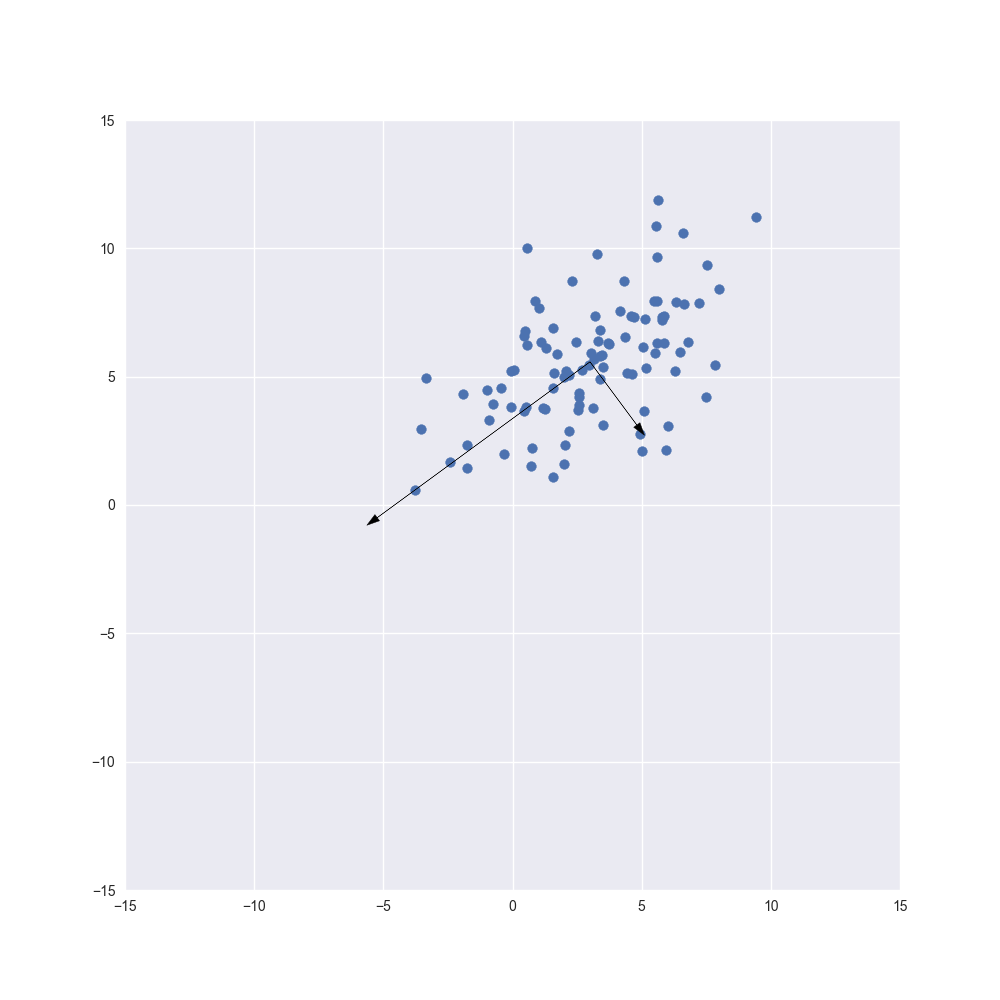
\includegraphics[width=300pt]{img/hw03_3d.png}
  \end{mdframed}

\item Let $U = \begin{bmatrix} v_1 & v_2 \end{bmatrix}$ be a $2 \times 2$
  matrix whose columns are the eigenvectors of the covariance matrix, where
  $v_1$ is the eigenvector with the larger eigenvalue. We use $U^{\top}$ as a
  rotation matrix to rotate each sample point from the $(X_1, X_2)$ coordinate
  system to a coordinate system aligned with the eigenvectors. (As
  $U^{\top} = U^{-1}$, the matrix $U$ reverses this rotation, moving back from
  the eigenvector coordinate system to the original coordinate system). Center
  your sample points by subtracting the mean $\mu$ from each point; then rotate
  each point by $U^{\top}$, giving $x_{\text{rotated}} = U^{\top}(x - \mu)$.
  Plot these rotated points on a new two dimensional-grid, again with both axes
  having range $[-15, 15]$.
  \begin{mdframed}
    \begin{minted}{python}
      U = evecs[:,::-1]
      X_centered = X - mu
      X_centered_rotated = (U.T @ X_centered.T).T

      fig = plt.figure(figsize=(10,10))
      plt.xlim(-15,15)
      plt.ylim(-15,15)
      plt.scatter(X_centered_rotated[:,0], X_centered_rotated[:,1])
    \end{minted}
    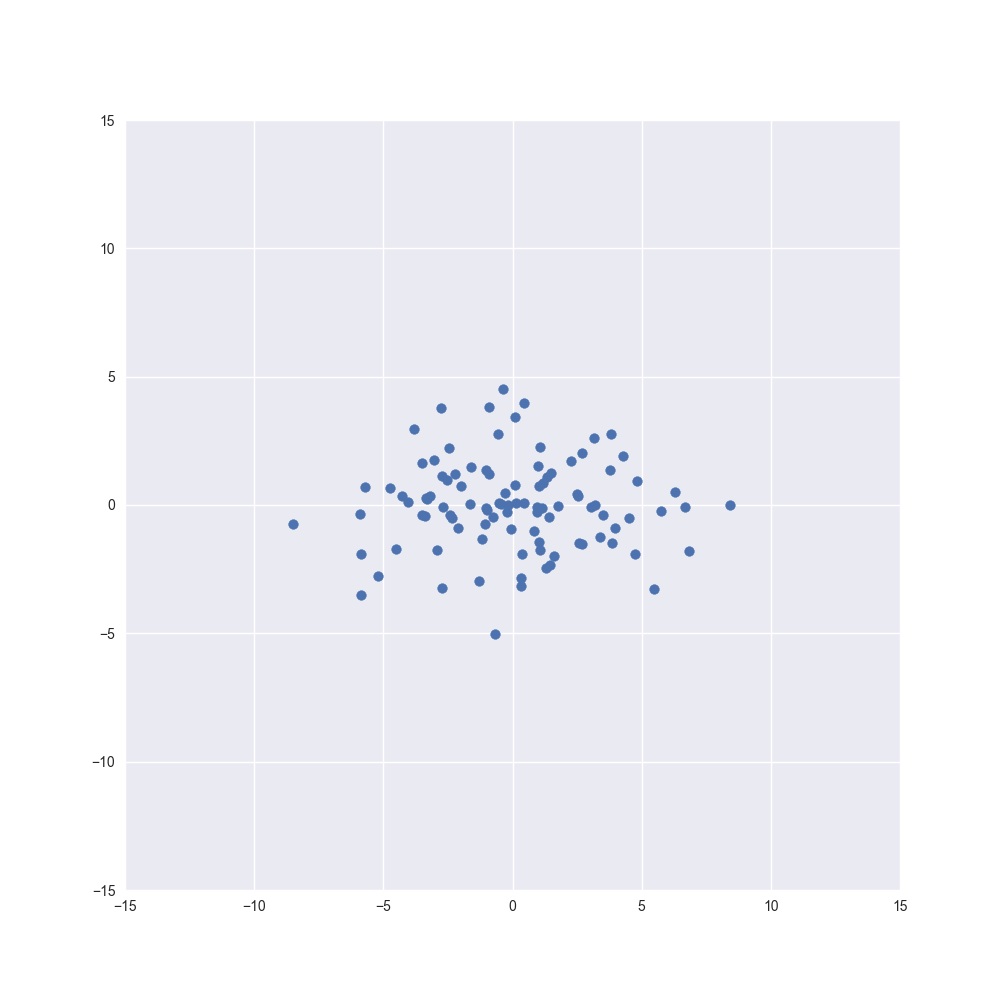
\includegraphics[width=300pt]{img/hw03_3e.png}
  \end{mdframed}

\end{enumerate}

\newpage
\subsection*{4. Maximum Likelihood Estimation}
Let $X_1, \ldots, X_n \in \R^d$ be $n$ sample points drawn independently from a multivariate normal distribution $\N(\mu, \Sigma)$.
\begin{enumerate}[label=(\alph*)]
    \item Suppose the normal distribution has an unknown diagonal covariance matrix
    $$
    \Sigma =
    \begin{bmatrix}
    \sigma_1^2 & & & & \\
    & \sigma_2^2 & & & \\
    & & \sigma_3^2 & & \\
    & & & \ddots & \\
    & & & & \sigma_d^2 \\
    \end{bmatrix}
    $$
    and an unknown mean $\mu$. Derive the maximum likelihood estimates, denoted $\hat{\mu}$ and $\hat{\sigma_i}$ for $\mu$ and $\sigma_i$. Show all your work.
    \begin{mdframed}
      First, let's get some intuition for the situation: the covariance matrix
      is diagonal, so the isocontours of the PDF of the Gaussian are
      axis-aligned. That means that the PDF can be factored into a product of
      one-dimensional marginal densities: i.e. we can compute the density of a
      sample vector $\vec x$ as the product of densities of its scalar
      components (individual features):
      $\p(\vec x;\vec \mu, \vec \Sigma) = \prod_{j=1}^d \p(\vec x_j; \mu_j,
      \sigma^2_j)$. We therefore expect the estimation problem to be fairly
      straightforward, essentially involving fitting $d$ one-dimensional
      Gaussians independently.

      The likelihood function is
      \begin{align*}
        \L(\mu, \Sigma)
        &= \prod_{i=1}^n \p(X_i;\mu, \Sigma) \\
        &= \prod_{i=1}^n \prod_{j=1}^d \p(\vec X_{ij}; \mu_j, \sigma^2_j) \\
        &= \prod_{i=1}^n \prod_{j=1}^d \frac{1}{(\sqrt{2\pi})^d \sigma_j^d} \exp\(\frac{-(X_{ij} - \mu_j)^2}{2\sigma_j^2}\), \\
      \end{align*}
      giving the log-likelihood function
      \begin{align*}
        \l(\mu, \Sigma)
        &= \sum_{i=1}^n \sum_{j=1}^d -d\log\sigma_j - \frac{(X_{ij} - \mu_j)^2}{2\sigma_j^2} + \constant \\
        &= \sum_{j=1}^d -nd\log\sigma_j - \frac{1}{2\sigma_j^2} \sum_{i=1}^n  (X_{ij} - \mu_j)^2  + \constant. \\
      \end{align*}
      Fix a particular feature $j$. The partial derivatives with respect to the
      mean and variance parameter for that feature are
      \begin{align*}
        \dldmuj &= \frac{1}{\sigma^2_j}\sum_{i=1}^n(X_{ij} - \mu_j) = \frac{1}{\sigma^2_j}\(-n\mu_j + \sum_{i=1}^nX_{ij}\)\\
        \dldsigmaj &= -\frac{nd}{\sigma_j} + \frac{1}{\sigma_j^3} \sum_{i=1}^n  (X_{ij} - \mu_j)^2.
      \end{align*}
      To find the MLE $\hat \mu_j$ we set the partial derivative equal to zero
      and solve for $\mu$:
      \begin{align*}
        \dldmuj = 0
        &\implies -n\hat \mu_j + \sum_{i=1}^nX_{ij} = 0\\
        &\implies \hat \mu_j = \frac{1}{n}\sum_{i=1}^nX_{ij}.
      \end{align*}
      To find the MLE $\hat \sigma_j$ we set the partial derivative equal to
      zero, set $\mu_j = \hat \mu_j$, and solve for $\sigma$:
      \begin{align*}
        \dldsigmaj = 0
        &\implies -nd + \frac{1}{\hat \sigma_j^2} \sum_{i=1}^n  (X_{ij} - \hat \mu_j)^2 = 0 \\
        &\implies \hat \sigma_j^2 = \frac{1}{nd}\sum_{i=1}^n  (X_{ij} - \hat \mu_j)^2.
      \end{align*}
      (Why is it valid to substitute $\hat \mu_j$ for $\mu_j$?)
    \end{mdframed}

    \begin{mdframed}
      To verify that these critical points are indeed maxima, we note first
      that $\l(\mu, \Sigma)$ is a quadratic in $\mu$, in which the sign of
      $\mu_j$ is negative. Therefore it is a concave-down quadratic in $\mu_j$
      and has only a maximum; no minimum.

      For $\sigma$ we compute the second partial derivative,
      \begin{align*}
        \ddldsigmajsigmaj = \frac{nd}{\sigma_j^2} - \frac{3}{\sigma_j^4} \SS_j,
      \end{align*}
      where $\SS_j = \sum_{i=1}^n  (X_{ij} - \mu_j)^2$, and evaluate it at the critical point:
      \begin{align*}
        \ddldsigmajsigmaj(\sigma_j)
        &= \frac{(nd)^2}{\SS_j} - \frac{3(nd)^4}{\(\SS_j\)^4} \SS_j\\
        &= \frac{(nd)^2}{\SS_j} - \frac{3(nd)^4}{\(\SS_j\)^3}.\\
      \end{align*}
      (I was expecting to be able to show that $\ddldsigmajsigmaj(\sigma_j)$ is
      negative but I don't seem to be managing to do so.)
    \end{mdframed}


  \item Suppose the normal distribution has a known covariance matrix $\Sigma$
    and an unknown mean $A \mu$, where $\Sigma$ and $A$ are known $d \times d$
    matrices, $\Sigma$ is positive definite, and $A$ is invertible.  Derive the
    maximum likelihood estimate, denoted $\hat{\mu}$, for $\mu$.
    \begin{mdframed}
      Let $\eta = A\mu$. Then $\hat \eta_j = \frac{1}{n}\sum_{i=1}^nX_{ij}$ as
      above.

      The likelihood function for $\mu$ is
      \begin{align*}
        \L(\mu)
        &= \prod_{i=1}^n \frac{1}{\(\sqrt{2\pi}\)^d\sqrt{|\Sigma|}}\exp\(-\frac{1}{2}(X_i - A\mu)^\T\Sigma^\1(X_i - A\mu)\),
      \end{align*}
      and the log-likelihood function is
      \begin{align*}
        \l(\mu) = -\frac{1}{2}\sum_{i=1}^n (X_i - A\mu)^\T\Sigma^\1(X_i - A\mu) + \constant.
      \end{align*}
    \end{mdframed}

\end{enumerate}

\newpage
\subsection*{5. Covariance Matrices and Decompositions}
As described in lecture, the covariance matrix $\text{Var}(R) \in \R^{d\times d}$ for a random variable $R \in \R^d$ with mean $\mu$ is
$$
\text{Var}(R) = \text{Cov}(R, R) = \E[(R- \mu)(R-\mu)^{\top}] =
\begin{bmatrix}
\Var(R_1) & \Cov(R_1, R_2) & \ldots & \Cov(R_1, R_d) \\
\Cov(R_2, R_1) & \Var(R_2) & & \Cov(R_2, R_d) \\
\vdots & & \ddots & \vdots \\
\Cov(R_d, R_1) & \Cov(R_d, R_2) & \ldots & \Var(R_d)
\end{bmatrix}
$$
where $\Cov(R_i, R_j) = \E[(R_i - \mu_i)(R_j - \mu_j)]$ and $\Var(R_i) = \Cov(R_i, R_i)$. \\

\noindent
If the random variable $R$ is sampled from the multivariate normal distribution $\N(\mu, \Sigma)$ with the PDF
$$ f(x) = \frac{1}{\sqrt{(2\pi)^d |\Sigma|}} e^{((x-\mu)^{\top}\Sigma^{-1}(x-\mu))/2},$$
then $\Var(R) = \Sigma$.\\

\noindent
Given $n$ points $X_1, X_2, \ldots, X_n$ sampled from $\N(\mu, \Sigma)$, we can estimate $\Sigma$ with the maximum likelihood estimator
$$ \hat{\Sigma} = \frac{1}{n} \sum_{i=1}^n (X_i - \mu)(X_i - \mu)^{\top},$$ which is also known as the covariance matrix of the sample
\begin{enumerate}[label=(\alph*)]
\item The estimate $\hat{\Sigma}$ makes sense as an approximation of $\Sigma$
  only if $\hat{\Sigma}$ is invertible. Under what circumstances is
  $\hat{\Sigma}$ not invertible? Make sure your answer is complete; i.e., it
  includes all cases in which the covariance matrix of the sample is
  singular. Express you answer in terms of the geometric arrangement of the
  sample points Xi.
    \begin{mdframed}
      Let $\dot X$ represent the centered data, i.e. $\dot X_i = X_i - \mu$.

      Note that $\hat \Sigma$ is the mean of a collection of $n$ outer product
      matrices $\dot X_i \dot X_i^\T$, where each outer product matrix is
      contributed by a single sample point. Also note that the columns of
      $\dot X_i \dot X_i^\T$ are all scalar multiples of $\dot X_i$.

      $\hat \Sigma$ is invertible if and only if it is full-rank. Full-rank
      means that its columns are linearly independent.

      From this point of view, the following circumstances will lead to
      $\hat \Sigma$ being singular:

      \begin{enumerate}
      \item \textbf{There is only one point.} If $n = 1$ then $\mu = X_1$ and
        $\dot X_1 = \vec 0$, and the outer product is the zero matrix. This is
        singular (e.g. determinant is zero).
      \item \textbf{$d > 1$ and there are only two points.} If $n = 2$ then
        $\mu$ lies on the line connecting the two points, so
        $\dot X_1 = a\dot X_2$ for some scalar $a$. Therefore the columns of
        the sum of the two outer product matrices differ only by a scalar
        multiple.
      \end{enumerate}

      In general, the centered sample vectors $\{\dot X_i: 1 < i \leq n\}$ must
      span $\R^d$. I.e. if the sample vectors lie in an affine hyperplane of
      $\R^d$ then $\hat \Sigma$ will be singular.

    \end{mdframed}

    \item Suggest a way to fix a singular covariance matrix estimator $\hat{\Sigma}$ by replacing it with a similar but invertible matrix. Your suggestion may be a kludge, but it should not change the covariance matrix too much. Note that infinitesimal numbers do not exist; if your solution uses a very small number, explain how to calculate a number that is sufficiently small for your purposes.
    \begin{mdframed} \solution
    % SOLUTION HERE
    \end{mdframed}

  \item Consider the normal distribution $\N(0, \Sigma)$ with mean $\mu =
    0$. Consider all vectors of length 1; i.e., any vector $x$ for which
    $|x| =1$. Which vector(s) $x$ of length 1 maximizes the PDF $f(x)$? Which
    vector(s) $x$ of length 1 minimizes $f(x)$? (Your answers should depend on
    the properties of $\Sigma$.) Explain your answer.
    \begin{mdframed}
      Let $\vec v_1, \vec v_2, \ldots, \vec v_n$ be unit-length eigenvectors of
      $\Sigma$, arranged in order of decreasing eigenvalue.

      Note that $f(x)$ is maximum at the mean $\vec 0$ and decreases with
      increasing distance from $\vec 0$. The exact form of this decrease is
      determined by the quadratic form
      $(\vec x - \mu)^\T\Sigma^\1 (\vec x - \mu)$.

      Then the unit vector $x$ that maximizes $f(\vec x)$ is $\vec v_n$. This
      is because the eigenvector with smallest eigenvalue points in the
      direction of least slope of the quadratic form. Similarly, $\vec v_1$ is
      the unit vector that minimizes $f(\vec x)$ because the eigenvector with
      largest eigenvalue points in the direction of greatest slope of the
      quadratic form.
    \end{mdframed}
\end{enumerate}

\newpage
\subsection*{6. Gaussian Classifiers for Digits and Spam}
In this problem, you will build classifiers based on Gaussian discriminant analysis. Unlike Homework 1, you are NOT allowed to use any libraries for out-of-the-box classification (e.g \texttt{sklearn}). You may use anything in \texttt{numpy} and \texttt{scipy}. \\

\noindent
The training and test data can be found on Piazza in the post corresponding to this homework. Don’t use the training/test data from Homework 1, as they have changed for this homework. Submit your predicted class labels for the test data on the Kaggle competition website and be sure to include your Kaggle display name and scores in your writeup. Also be sure to include an appendix of your code at the end of your writeup.

\begin{enumerate}[label=(\alph*)]
    \item Taking pixel values as features (no new features yet, please), fit a Gaussian distribution to each digit class using maximum likelihood estimation. This involves computing a mean and a covariance matrix for each digit class, as discussed in lecture. \emph{Tip}: You may, and probably should, contrast-normalize the images before using their pixel values. One way to normalize is to divide the pixel values of an image by the $l_2$ norm of its pixel values.
    \item (Written answer) Visualize the covariance matrix for a particular class (digit). How do the diagonal terms compare with the off-diagonal terms? What do you conclude from this?
    \begin{mdframed} \solution
    % SOLUTION HERE
    \end{mdframed}

    \item Classify the digits in the test set on the basis of posterior probabilities with two different approaches.
    \begin{enumerate}[label=(\roman*)]
        \item Linear discriminant analysis (LDA). Model the class conditional probabilities as Gaussians $\N(\mu_C, \Sigma)$ with different means $\mu_C$ (for class C) and the same covariance matrix $\Sigma$, the average covariance matrix of the 10 classes. \\

        Hold out 10,000 randomly chosen training points for a validation set. Classify each image in the validation set into one of the 10 classes (with a 0-1 loss function). Compute the error rate and plot it over the following numbers of randomly chosen training points: $$[100, 200, 500, 1,000, 2,000, 5,000, 10,000, 30,000, 50,000].$$ (Expect some variance in your error rate when few training points are used.)

        \item Quadratic discriminant analysis (QDA). Model the class conditionals as Gaussians $\N(\mu_C, \Sigma_C)$, where $\Sigma_C$ is the estimated covariance matrix for class C. (If any of these covariance matrices turn out singular, implement the trick you described in Q5.(b). You are welcome to use $k$-fold cross validation to choose the right constant(s) for that trick.) Repeat the same tests and error rate calculations you did for LDA.

        \item  (Written answer.) Which of LDA and QDA performed better? Why?
        \begin{mdframed} \solution
        % SOLUTION HERE
        \end{mdframed}

        \item Train your best classifier with \texttt{train.mat} and classify the images in \texttt{test.mat}. Submit your labels to the online Kaggle competition. Record your optimum prediction rate in your submission. You are welcome to compute extra features for the Kaggle competition. If you do so, please describe your implementation in your assignment. Please use extra features \textbf{only} for this portion of the assignment. In your submission, include plots of error rate versus number of training examples for both LDA and QDA. Also include tables giving the error rates (as percentages) for each number of training examples for both LDA and QDA. Include written answers where indicated.
        \begin{mdframed} \solution
        % SOLUTION HERE
        \end{mdframed}

    \end{enumerate}
    \item Next, apply LDA or QDA (your choice) to spam. Submit your test results to the online Kaggle competition. Record your optimum prediction rate in your submission. If you use additional features (or omit features), please describe them. \\

    \emph{Optional:} If you use the defaults, expect relatively low classification rates. The TAs suggest using a bag-of-words model. You may use third-party packages to implement that if you wish. Also, normalizing your vectors might help.

    \begin{mdframed} \solution
    % SOLUTION HERE
    \end{mdframed}

    \item \emph{Extra for Experts:} Using the \texttt{training\_data} and \texttt{training\_labels} in \texttt{spam.mat}, identify 10 words in your features set corresponding to the maximum and minimum variances. Use $k$-fold cross validation to train your classifier using only 10 variance-maximum words and record your average error rate. Do the same with the 10 minimum-variance words. What do you notice?
    \begin{mdframed} \solution
    % SOLUTION HERE
    \end{mdframed}
\end{enumerate}

\end{document}
